\begin{example}[title = Undecidability halting problem]
    \textbf{Problem}. \\
    Prove the undecidability of the \textbf{halting problem}, namely the fact that the following function
    $$ halt(\alpha, x) = \begin{cases} 1 \text{ if } M_{\alpha}(x) \text{ terminates } \\ 0 \text{ otherwise }\end{cases} $$
    is \textbf{not computable}. \vspace{14pt}

    \textbf{Note}. \\
    For this kind of problem, we have two different ways to solve it:
    \begin{itemize}
        \renewcommand{\labelitemi}{-}
        \item \textbf{reduction}, reducing the proof to a well-known existing problem already uncomputable;
        \item \textbf{directly}, solving it.
    \end{itemize}
    We use a technique that lies between the ones presented, exploiting a well-known problem that is already undecidable (\textit{namely the uc function}). \vspace{14pt}

    \textbf{Observations}.
    \begin{itemize}
        \renewcommand{\labelitemi}{-}
        \item We want to prove that the computational task \textit{halt} is undecidable.
        \item The main assumption of the proof is that we know for sure that it's impossible to build a machine that computes \textit{halt}.
        \item We start saying that exists a Turing Machine able to compute the \textit{halt} function and then we get a contradiction about our original thesis.
    \end{itemize} \vspace{14pt}

    \textbf{Solution}. \\
    We show that from a hypothetical machine computing the function \textit{halt}, call it $M_{halt}$, we can build another machine $M_{uc}$ which computes function
    \textit{uc}. Since we know such a machine cannot exists (\textit{by definition the uc function is uncomputable}), we are done. \vspace{7pt}

    Described the main idea, we need to use $M_{halt}$ as a subroutine in building $M_{uc}$, so the \textit{halt} function is an inner piece of $M_{uc}$ 
    in our construction of the function \textit{uc}. \vspace{7pt}

    Let's construct $M_{uc}$ using $M_{halt}$ as a subroutine. \vspace{7pt}

    On input $\alpha$ the machine $M_{uc}$ proceeds as follows:
    \begin{enumerate}
        \item We call $M_{halt}$ on input $(\alpha, \alpha) \in \{0,1\}^*$, where $x$ is equal to $\alpha$.
        \item We wait until $M_{halt}$ returns the output.
        \item We proceed in two different ways than the output returned by $M_{halt}$:    
        \begin{enumerate}
            \item If $M_{halt}$ returns $0$ on input $(\alpha, \alpha)$, meaning that $M_{\alpha}(\alpha)$ does not terminate (\textit{we are in the second case of uc where $M_{uc}$ returns 1}).
            \item If $M_{halt}$ returns $1$ on input $(\alpha, \alpha)$, $M_{uc}$ knows that it can safely call \textit{U}, the Universal Turing Machine, on input $(\alpha, \alpha)$, since $M_{\alpha}(\alpha)$ terminates and thus $U(\alpha, \alpha)$ terminates too. Therefore, let's then call $U(\alpha, \alpha)$ and let $b$ be the answer we receive (\textit{we are using U as $M_{\alpha}$, since $U(x, \alpha) = M_{\alpha}(x)$ by definition}).
        \end{enumerate}
        \item We return the negation of $b$, as follows:
        \begin{enumerate}
            \item If $b = 1$, then $M_{\alpha}(\alpha) = 1$, and $uc(\alpha) = 0$ by definition.
            \item If $b = 0$, then $M_{\alpha}(\alpha) = 0$, and $uc(\alpha) = 1$ by definition.
        \end{enumerate}
        \item The way we have defined $M_{uc}$ ensures that it computes the function \textit{uc}, in particular relying on the fact that $M_{halt}$ solves the computational task \textit{halt} and $U$ is the Universal Turing Machine.
    \end{enumerate} \vspace{14pt}

    \textbf{Final mark}. \\
    Since such machine $M_{uc}$ does not exist, also $M_{halt}$ does not exist in the first place, therefore we have done. $\square$ \vspace{14pt}

    \textbf{Note}. \\
    Why do we introduce the Universal Turing Machine $U$ inside the proof?
    
    Giving in input $(\alpha, \alpha)$ to the Turing Machine $M_{halt}$ tells us only if the computation stops or proceeds, it doesn't give us the exact result. Therefore,
    when the computation finally stops, $M_{halt}$ does not give us any information about the result. So, we need the Universal Turing Machine in order to simulate
    $M_{halt}$ over $\alpha$ to achieve the final answer, that in this case it could be $y \in \{0,1\}$.
\end{example}
\begin{example}[title = Haltstar problem]
    \textbf{Problem}. \\
    Given the following function
    \[
        \mathit{haltstar}(s) = 
            \begin{cases} 
                1 & \text{if } s = \lfloor \alpha, x_1, \dots, x_n \rfloor \wedge M_{\alpha}(x_1) \wedge \dots \wedge M_{\alpha}(x_n) \text{ terminates} \\
                0 & \text{if } s = \lfloor \alpha, x_1, \dots, x_n \rfloor \wedge \exists i \in \{1, \dots, n\} \text{ s.t. } \\
                & M_{\alpha}(x_i) \text{ does not terminate}
            \end{cases}
    \]

    is it computable or uncomputable? \vspace{14pt}

    \textbf{Note}.
    \begin{itemize}
        \renewcommand{\labelitemi}{-}
        \item We do not check the termination condition only on one input, but over many inputs $x_1, \dots, x_n$.
        \item We name $L_{haltstar}$ the language underlining the \textit{haltstar} function, putting in relation the problem $L_{haltstar}$ with an already known undecidable problem.
    \end{itemize} \vspace{14pt}

    \textbf{Observations}.
    \begin{itemize}
        \renewcommand{\labelitemi}{-}
        \item The whole thing is just being able to frame the problem in the following way: $$ s \in G \rightarrow \phi(s) \in L $$
    \end{itemize} \vspace{14pt}

    \textbf{Solution}. \\
    We prove \textit{haltstar} to be \textbf{uncomputable}, showing $L_{haltstar}$ is undecidable (\textit{$L_{haltstar}$ is the set of strings on which 
    haltstar returns $1$}). The latter can be proved by reduction from the undecidability of $L_{halt}$ (\textit{reducing the proof to a problem that 
    we already know to be uncomputable}). \vspace{7pt}

    We have to define, in other words, a function as follows 
    $$ \phi: \{0,1\}^* \rightarrow \{0,1\}^* $$
    such that two constraints are satified:
    \begin{enumerate}
        \item $\phi$ is computable.
        \item $s \in L_{halt} \Leftrightarrow \phi(s) \in L_{haltstar}$
    \end{enumerate} \vspace{7pt}

    We define $\phi$ as follows:
    $$ \lfloor (\alpha, x) \rfloor \xrightarrow{\phi} \lfloor \alpha, x \rfloor $$
    so, $\phi$ it's just an identity function, a way to encode pairs to tuples. Anyway, the encoding done by this function it's a litte bit different than what 
    we have seen so far, in particular:
    \begin{itemize}
        \renewcommand{\labelitemi}{-}
        \item $\lfloor (\alpha, x) \rfloor \rightarrow$ encoding of pairs
        \item $\lfloor \alpha, x \rfloor \rightarrow$ encoding of tuples
    \end{itemize} \vspace{7pt}

    We can state:
    \begin{itemize}
        \renewcommand{\labelitemi}{-}
        \item $\phi$ is easily seen to be computable, it does nothing besides playing with encoding of pairs and tuples.
        \item moreover 
        \[
            s \in L_{\text{halt}}
            \begin{aligned}[t]
                & \Leftrightarrow s = \lfloor (\alpha, x) \rfloor M_{\alpha}(x) \text{ terminates} \\
                & \Leftrightarrow \phi(s) = \lfloor \alpha, x \rfloor M_{\alpha}(x) \text{ terminates} \\
                & \Leftrightarrow \phi(s) = \lfloor \alpha, x_1, \dots, x_n \rfloor \wedge n = 1 \wedge M_{\alpha}(x_i) \\ 
                & \qquad \text{ terminates } \forall i \in \{1, \dots, n\} \\
                & \Leftrightarrow \phi(s) \in L_{haltstar}
            \end{aligned}
        \]
    \end{itemize} \vspace{14pt}

    \textbf{Final mark}. \\
    This sequence of double implications is extremely pedantic, but we need it to convince us that we are not cheating. Therefore, we started from the more general 
    undecidable problem $L_{halt}$ coming to the less general, proving that also the more specific one $L_{haltstar}$ is undecidable.
\end{example}
\begin{example}[title = $inc(x)$ function]
    \textbf{Problem}. \\
    Show that the function $inc: N \rightarrow N$ such that $inc(x) = x + 1$ can be computed by a Turing Machine and it works in linear time. \vspace{14pt}

    \textbf{Note}. 
    \begin{itemize}
        \renewcommand{\labelitemi}{-}
        \item Encoding in a Turing Machine works on strings and the given function works within natural numbers.
        \item We have to build a Turing Machine, since it's intrinsically asked.
    \end{itemize} \vspace{14pt}.

    \textbf{Observations}. \\
    Let's take a look about how the machine behaves before the solution. \vspace{7pt}

    Like the image below, we start from the right-side tape and we would like something as on the left-side tape. \vspace{3.5pt}
    \begin{center}
        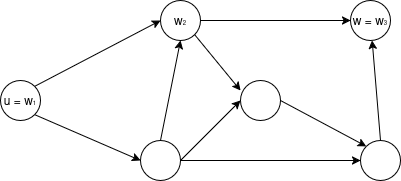
\includegraphics[width=0.7\textwidth]{img/img1.png}
    \end{center} \vspace{3.5pt}

    Building such a Turing Machine it's quite easy: we move the tape head to right, until it reaches the last binary symbol and we can start encrease by $1$. \vspace{7pt}

    However, if we suppose a little bit more annoying binary number as follows: \vspace{3.5pt}
    \begin{center}
        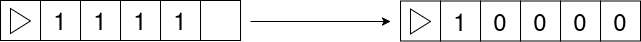
\includegraphics[width=0.7\textwidth]{img/img2.png}
    \end{center} \vspace{3.5pt}

    the construction of the Turing Machine seems to be more difficult than before. \vspace{7pt}

    \textbf{What shall we do?}
    \begin{enumerate}
        \item Insist with this kind of encoding.
        \item Use the \textbf{reverse encoding}. \\
        For instance, by reverse encoding the first binary number $1100$ would be $0011$ and just modifying the first occurence $0$, turning it to $1$, we could
        terminate the computation. In the second case the reverse enconding doesn't help us, since $1111$ would remain unchanged. Anyway, reasoning with this 
        approach, from the left to the right, we know for sure that we have something to carry until we reach a blank cell.
        \vspace{3.5pt}
        \begin{center}
            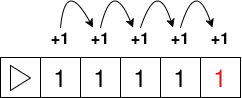
\includegraphics[width=0.3\textwidth]{img/img3.png}
        \end{center} \vspace{3.5pt}
    \end{enumerate} \vspace{14pt}

    \textbf{Solution}. \\
    Any possible Turing Machine is described by the triple $M = (\Gamma, Q, \delta)$, where each of them in this solution are composed by:
    \begin{itemize}
        \renewcommand{\labelitemi}{-}
        \item $Q = \{q_{init}, q_0, q_1, q_{halt}\}$
        \item $\Gamma = \{\square, \triangleright, 0, 1\}$
        \item $\delta$ = 
            \begin{itemize}
                \renewcommand{\labelitemi}{}
                \item $(q_{init}, \triangleright) \rightarrow (q_0, \triangleright, R)$
                \item $(q_{0}, 0) \rightarrow (q_1, 1, L)$
                \item $(q_{0}, 1) \rightarrow (q_0, 0, R)$
                \item $(q_{0}, \square) \rightarrow (q_1, 1, L)$
                \item $(q_{1}, 0) \rightarrow (q_1, 0, L)$
                \item $(q_{1}, 1) \rightarrow (q_1, 1, L)$
                \item $(q_{1}, \triangleright) \rightarrow (q_{halt}, \triangleright, S)$
                \item $(q_{halt}, \triangleright) \rightarrow (q_{halt}, \triangleright, S)$
            \end{itemize}
    \end{itemize}
    where:
    \begin{itemize}
        \renewcommand{\labelitemi}{-}
        \item $q_0 \rightarrow$ state before changing the binary number
        \item $q_1 \rightarrow$ state after changing the binary number
    \end{itemize} \vspace{14pt}

    \textbf{Observations}.
    \begin{itemize}
        \renewcommand{\labelitemi}{-}
        \item Some transitions are not listed, for instance $(q_{halt}, 0)$ or $(q_1, \square)$, we didn't specify them. These more precise cases seem to be more harmless: even though we describe in details every single transition, our machine still works as before. Therefore, we can suppose that these additional cases will never occur.
        \item Some states are meaningful only when they are related to specific symbols (\textit{e.g. $q_{init}$ within the starting symbol $\triangleright$}).
    \end{itemize}
\end{example}